\chapter{The TLS Echo Web Service}

The Web Services of the previous chapters have one major drawback: the communication between the two endpoints is insecure.
For that reason the current and the next chapters will discuss how to create a secure Web Service.
In general, security in a network can be subdivided into the following categories:~\cite{TANNENBAUM_2001}\task{TODO: verfiy this citation}
\begin{itemize}
	\item \textbf{Confidentiality} --- Protection of the data against passive attacks (such as publicise message content)
	
	\item \textbf{Authentication} --- Verification of the identity of the communication partners.

	\item \textbf{Integrity} --- Protection against interception and manipulation, replay, insertion, etc.  of a message.

	\item \textbf{Non-repudiation} --- Preventing the sender to repudiate the message transmitted by him.

	\item \textbf{Access control} --- Restrict the access to ressources.

	\item \textbf{Availability} --- Ensure a system is always usable which is challenged by various attacks.

\end{itemize}
%1-21   Gebräuchliche Dienste
%     Identifizierung           Vermerk
%     Berechtigung              Zugriff
%     Lizenz/Zertifizierung     Gültigkeitsprüfung
%     Unterschrift              Zeitpunkt des Auftretens
%     Bezeugung                 Abstimmung
%     Übereinstimmung           Eigentum
%     Zuverlässigkeit           Registrierung
%     Quittungen                Genehmigung/Verbot
%     Bestätigung des Ursprungs Privatsphäre
%
% Nach Sicherheit in verteilten Systemen, ITM Lübeck
Ideally, all six categories should have been achieved by such an application (though the last category, availability, is difficult to realise).
In the present chapter, the security will be put into practice by extending the protocol stack with an additional security layer called TLS (Transport Layer Security).
Due to the location between the TCP and the HTTP layer, the layer is only capable to limit the access of the grid to a certain set of users. Once the user has passed the layer sucessfully, all resources provided by the HED are available. This kind of behaviouor can be seen as to be very coarse grained.
Nevertheless, it provides the security categories: confidentiality, authentication, integrity, non-repudiation and access control.\\


The next section gives a basic understanding of the working principle of the TLS. In order to enable newcomers an entry to  this area, emphasis is put on the security concept and not on an exact description of the technical realisation.


% It is recommand to satifiy as much categories as possible. 
%authentication , confidentiality and integrity protection of TCP-based communication --- non-repudiation due to private key, access control to our service.


\section{Transport Layer Security}


The TLS is a protocol which provides a secure connection between two endpoints.
It is based directly on the TCP/IP layers and uses typically an asymmetric encryption to establish the connection (alternatively a symmetric pre-shared key may be used).
After the communication has been successfully established, both participants are switching to another encryption method which is based on a new negotiated symmetric key.\\
%    1. Peer negotiation for algorithm support
%    2. Key exchange and authentication
%    3. Symmetric cipher encryption and message authentication   - from wikipedia
%
%


Symmetric and asymmetric encryption are the two main classes of cryptographic algorithms.
In case of symmetric encryption, both participants are holding the same secret key to encrypt and decrypt a plain text.
The principle is to reverse the process of encryption in order to decrypt the text.
Symmetric encryption can be ranked as being very secure but its downside is that the key distribution is very difficult in practice.
The key has to be shared previously, ideally over a secure channel which may either be a complete different medium (i.e. a letter or speech) or a channel which has been encrypted with another secret key.
Asymmetric encryption follows a different functional principle.
While the symmetric encryption utilise one key, the asymmetric ecryption is based on two keys: a private key and public key.
As the names imply, the private key is kept secret and is never revealed to others while the public key is available for everyone.
Messages encrypted with the public key can only be decrypted with the private key and conversely, messages encrypted with the private key can only be decrypted with the public key. 
The Figure~\ref{fig:asymmetric_encryption} illustrates the circumstances of the case.\\
\begin{figure}[htb]
	\centering%epstopdf async.eps
	\subfloat[\textbf{A plain text which has been encrypted with the private key can only be decrypted with the public key.}
		If the receivers is sure that the public key is related to a certain identity, 
			the private key can be used to sign the messages.
		Only the owner of the private key is able to create encrypted messages which can be decrypted with the public key. \label{fig:cgd}]
		{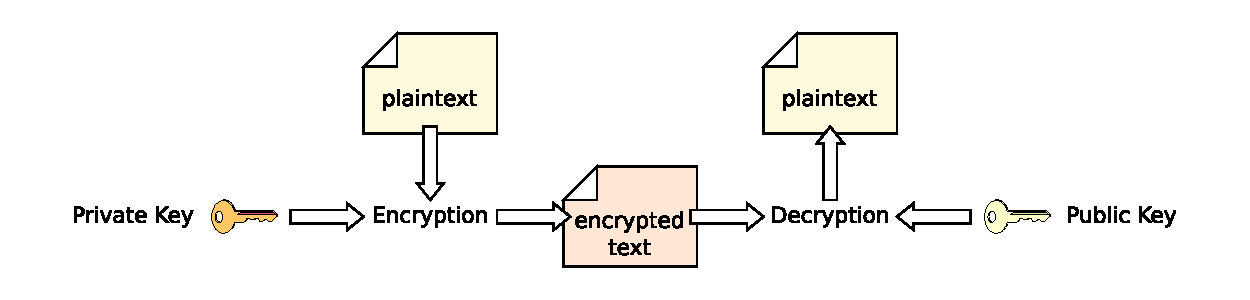
\includegraphics[width=12cm]{tex_tls_echoservice/async.pdf}}\\
	\subfloat[\textbf{A plain text which has been encrypted with the public key can only be decrypted with the private key.}
		Using asymmetric keys in that manner offers the possiblity to send encrypted messages to the owner of the private key.
		\label{fig:cgd2}]
		{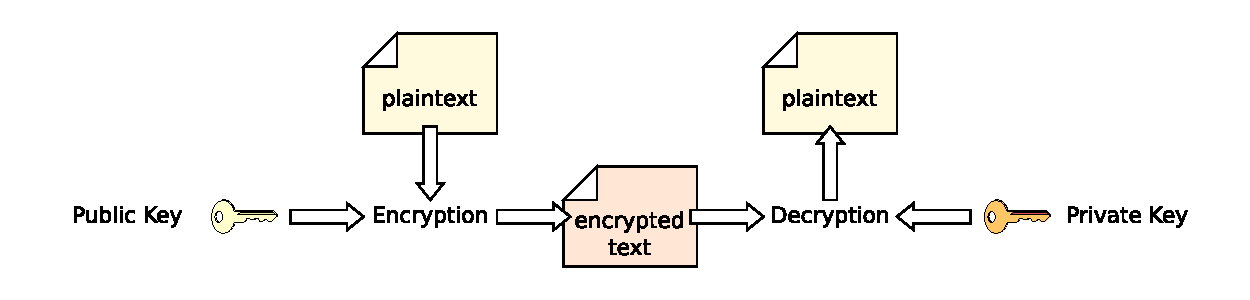
\includegraphics[width=12cm]{tex_tls_echoservice/async2.pdf}}
	\label{fig:asymmetric_encryption}
	\mycaption{Usage of asymmetric encryption.}{}
\end{figure}


At startup of a communication process, A (Alice) who desires a secure connection transmits her public key to B (Bob).
Bob is now able to encrypt his messages such that only Alice is able to decrypt them.
As one can see, this first approach already provides confidentiality and integrity of messages.
But neither non-repudiation, authentication and consequently nor access control are established because the identity of Alice is not proven.
In order to be able to check identities, so called certificates have been invented.
Certificates render the possibility to validate the identity of its owner.
They are signed by a certificate authority (CA), the identity of which can be verified by another CA or that is pre-configured to be trusted.\\


A certificate is composed of the identity of its owner, its public key, the name of the CA who signed the certificate and the signature of the CA which is a hash-value of the certificate encrypted with the private key of the CA. 
Furthermore, the algorithms used to create the certificate are added.
If a certificate can be resolved to a trusted CA, the identity of the certificate owner is considered to be proven. 
In general, a set of trusted CAs is already defined in the operation system.
To obtain a certificate, a certificate request has to be submitted to a CA.
The CA verifies the identity of the requesting person and the requested certificate will be signed.
Figure~\ref{fig:certificate_request} shows the procedure of gaining a certificate.
For instructions on the actual commands on the UNIX shell, you may follow instructions on \url{http://ca.nordugrid.org}.
\begin{figure}[htb]
	\centering%epstopdf certificates.eps
 	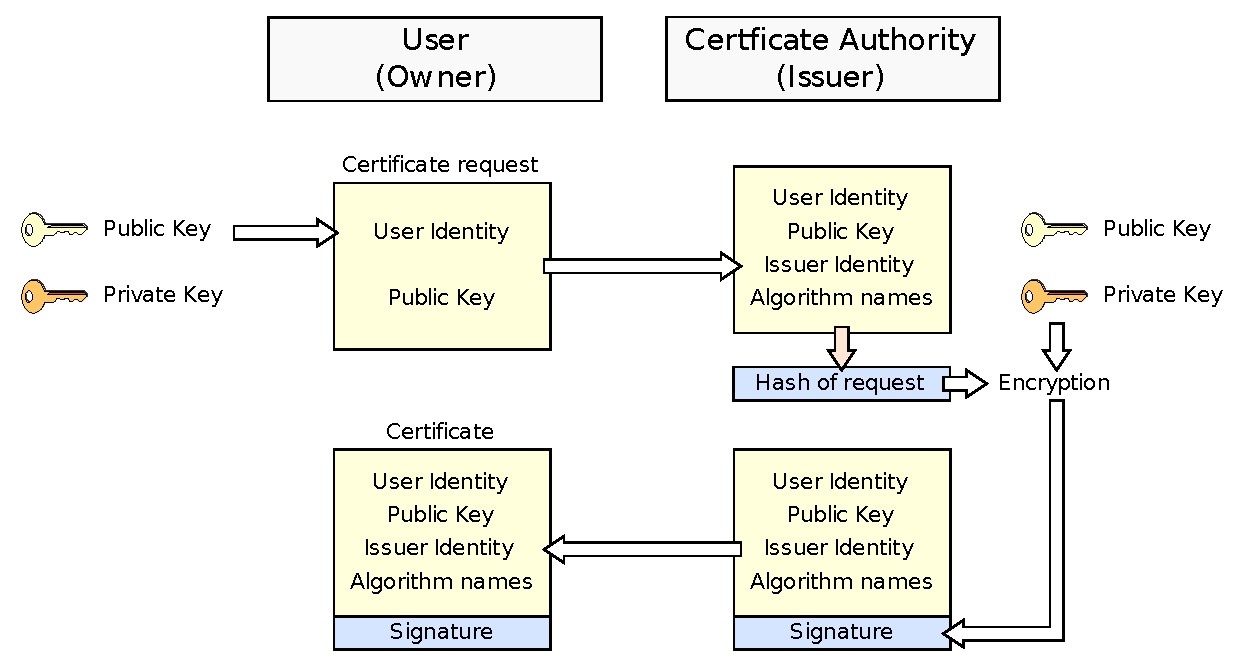
\includegraphics[width=13cm]{tex_tls_echoservice/certificates.pdf}
	\mycaption{Procedure of certificate signing.}{}
	\label{fig:certificate_request}
\end{figure}
In the first step, a private and a public key will be generated by the requester.
The public key together with a textual description of the identity depict the request which will be transmitted to a CA.
After the CA successfully verified the validity of the request, the identity of the CA and the name of the used encryption algorithms are added.
The collected data will represent the plain text of the certificate.
In order to ensure the integrity of the text, a hash value will be created.
This is a fixed-sized short string which is generated by an algorithm based on an arbitrary long given text.
The algorithm is designed such that a small change in the text will cause the hash value to change almost like a random function.
Thus, the hash value can be used a fingerprint of the text.
The CA signs the plain certificate by encrypting its hash value with its private key.
Finally the signed certifcate will be returned to the requester.
If an outside person wants to verify the certificate owner, the encrypted hash value has to be decrypted by the public key of the CA and a hash value has to be created with the same algorithm in order to compare them.\\


Figure~\ref{fig:verification_of_certificates} shows a usecase in which Alice wants to resolve the identity of Bob.
Alice submits her request to Bob along with a challange consisting of a random number $n$. 
Bob encrypts the number with his private key and returns it together with his certificate.
The random number ensures that it is not possible to repeat a message (integrity) and to prove that the communication partner holds the private key.
Alice uses the public key of Bob to decrypt the challenge. 
If the decrypted number is equal to the transmitted number, Alice can reason that the identity of Bob is to be trusted in case she is trusting the CA which has signed Bobs certificate.\\

In the given example, Alice only trusts the CA 2 but not CA 1.
To resolve the identity of CA 1, Alice establishes a connection to CA 1 and submits another random number $n$ as a challenge.
The CA 1 encrypts the challenge with its private key and sends the result along with its certificate back to Alice. 
Alice successfully compares the returned number. Additionally she validates the certificate of CA 1 with the pre-configured certificate of CA 2..
Since the certificate was signed by CA 2 which is pre-configured to be trusted, she also trusts CA 1 and in conclusion the identity of B.
In summary, Alice knows she is talking to Bob.
If Bob also wants to be sure who he's talking to, then the same procedure has to be done to confirm the identity of Alice.
The TLS mode in which both endpoints are ensuring themselves to whom they are talking to is called \textit{bilateral connection mode}.\\


When the client is aware of the server's authentity, the confidential treatment of its data is guaranteed such that one can be sure the data won't be revealed to a third party (server-sided confidentiality). 
On the other side, if the server is aware of the client authentity, the access to services and resources can be controlled (access control). Thus, in case of services, the results will only be passed back to the right person (client-sided confidentiality). 
As one can see confidentiality, authentication, integrity and non-repudiation are now established.\\

\begin{figure}[tbh]
	\centering%epstopdf verification.eps 
	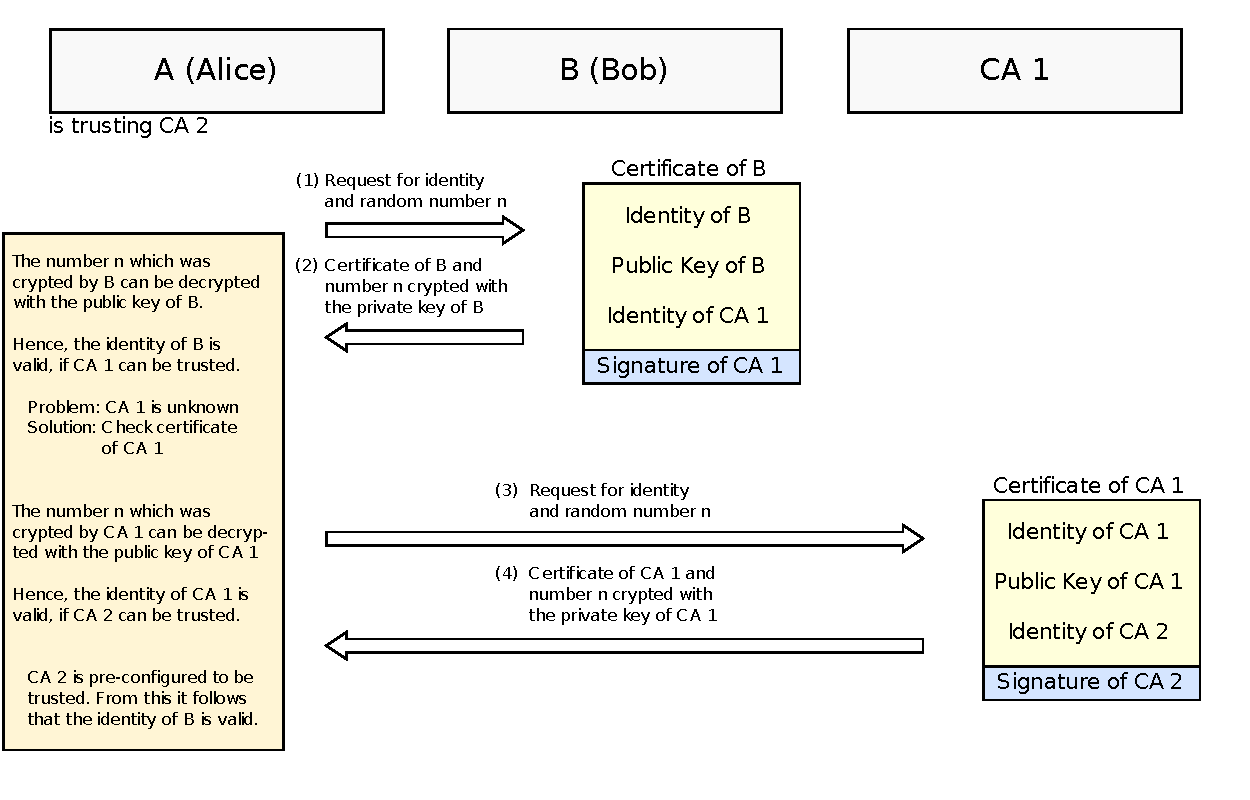
\includegraphics[width=13cm]{tex_tls_echoservice/verification.pdf}
	\mycaption{Usecase in which Alice resolves the identity of Bob.}{In order to resolve the identity of Bob, Alice sends a request for Bob's identity along with a newly created random number to Bob. Bob encrypts the received number using his private key and returns his public key to Alice. Due to the random number can only be encrypted by the owner of the private key, Alice is able ot verify that the certificate was transmitted by his owner. Since the certificate was signed by the CA 1, which she is not per-configured to be trust, Alice needs to resolve also the identity of CA 1. The request is done in the same manner, but this time the certificate is signed by the trusted CA 2. Due to the fact she is now able to trust CA 1, Alice can now also trust the identity of Bob.}
	\label{fig:verification_of_certificates}
\end{figure}

Certificates have several advantages.
They are scaling very good with the amount of users because CAs can create new sub-CAs such that the load is balanced (certificates of a CA may be cached).
Furthermore, no critical information is exchanged for the establishment of a connection (in particular: no secret key is shared which may get intercepted).
Instead, a set of pre-configured CAs which will be in general provided by the operation system is needed.
In respect of ARC it is obvious that the access to the grid shall be under the control of its administrator.
To do so, the administrators have to create their own CAs which are in charge of creating certificates for new users.
The identity of the created CA has to be added to the directory of pre-configured CAs.
Many universities have prepared local certificate authorities. And every user can establish his own. Certificates in general, however, have found entry to regular computer users, for instance with the FernUniversity Hagen (https://ca.fernuni-hagen.de/) who use that technology for their remote students to hand in exercises.\\


A CA which controls access to a grid can be considered as a virtual organsiation (VO).
It may involve organisations close to the leading organisation as well as structure which are not formally associated with it.
In most cases the basic idea is to share ressources. \task{this para will need some overhaul - SM; jup, that a bit short... unfortunatly I am not very familiar with that stuff, but I am on it :-( - MG}

\clearpage
\section{Service}


In order to create a secure connection we hence need two certificates: a client certificate and a service certificate.
The CA of the certificate has to be pre-configured on the counterpart and furthermore, the owner of the certificate has to hold the fitting private key.
For the given example X.509-certificates in the PEM format will be used which are standardised by the ITU-T.
Altogether six files are needed:\\
\\
\begin{tabular}{l@{~---~}p{13cm}}
\textbf{clientCA}   & The CA which guarantees for the identity of the client \\
\textbf{clientCERT} & The certificate of the client. \\
\textbf{clientKEY}  & The private key of the client (should be kept in safe custody).\vspace{2ex}\\
\textbf{serverCA}   & The CA which guarantees for the identity of the server \\
\textbf{serverCERT} & The certificate of the server. \\
\textbf{serverKEY}  & The private key of the server (should be kept in safe custody).\\
\end{tabular}
\forcelinebreak
\\






To get this service running, the six files have to be distributed. The server should hold the files: serverCERT.pem, serverKEY.pem and clientCA.pem. The client on the other side should own the files: clientCERT.pem, clientKEY.pem and serverCA.pem.
Within the source code directory that accompanies this document certificates with corresponding names are prepared. Due to certificates have a limited period of validity, these certificates may no longer be accepted by the communication parter.
One has to create new certificates to ensure the proper work of the TLS Web Service.\\


Several tools are available which allow the handling for more advanced UNIX users. In order to create a first basic set of certificates signed by a self created CA, the shell scripts \textit{createMasterCA.sh} and \textit{createSlaveCert.sh} can  be found within the directory \textit{src/services/tlsechoservice/certFactory} may be used. The script \textit{createMasterCA.sh} will create a new CA and will overwrite older ones. The script \textit{createSlaveCert.sh} creates several certificates signed by the CA.\\


The TLS Echo Web Service implementation is almost the same as the one presented in the previous chapter. Merely the Class name and the namespace of the service have been changed. The only modification is done within the server configuration file which is displayed in Listing~\ref{lst:tls_echo_arched_xml}.
\lstsetARCHEDXML
\lstinputlisting
	[
	label=lst:tls_echo_arched_xml,float=htb,
	caption={[HED configuration file for the Arc intern echo service. Filename: arcecho\_no\_ssl.xml]
	\textbf{HED configuration file for the Arc intern echo service. Filename: arcecho\_no\_ssl.xml\textcolor{white}{hmf}}}
	]
{../examples/src/services/tlsechoservice/arched_tls_echoservice.xml}
The first change is in line~\ref{lst_code:tls_echo_arched_xml_plugin}. As to be seen, another plugin called \textit{mcctls} will be loaded by the \textit{ModuleManager}. The second change is the new element which has been placed between the TCP and the HTTP component, see line~\ref{lst_code:tls_echo_arched_xml_component}. Within the TLS element the certificates can be declared using the elements \textit{KeyPath}, \textit{CertificatePath}, \textit{CACertificatePath} and \textit{CACertificatesDir}.
% \begin{verbatim}
% <KeyPath>./clientKey.pem</KeyPath>
% 
% <CertificatePath>./clientCert.pem</CertificatePath>
% 
% <CACertificatePath>./serviceCA.pem</CACertificatePath>
% 
% <CACertificatesDir>/etc/grid-security/certificates</CACertificatesDir>
% \end{verbatim}
% or
% \begin{verbatim}
% <ClientSSLConfig FromFile='filename'/>
% \end{verbatim}
% \task{You can put the ClientSSLConfig into a separate file, then use <ClientSSLConfig FromFile='filename'/> in each service, and then you don't need to change everywhere - proposed by Zsombor - but I can't find any example *hrmlgrmpf*...}


%\lstsetCPP
%\lstinputlisting
%	[
%	label=lst:tls_echo_service_cpp,
%	caption={[HED configuration file for the Arc intern echo service. Filename: arcecho\_no\_ssl.xml]
%	\textbf{HED configuration file for the Arc intern echo service. Filename: arcecho\_no\_ssl.xml\textcolor{white}{hmf}}}
%	]
%{../examples/src/services/tlsechoservice/tlsechoservice.cpp}
%
% Lassen wir mal weg....
%
%
% \lstsetKSH
% \begin{lstlisting}[
% label=lst:tls_echo_arched_invoke,float=htb,
% caption={[Transformation in eine uniforme konzentrische Verteilung.]
%          \textbf{Transformation in eine uniforme konzentrische Verteilung.\textcolor{white}{hmf}}}]
% $ rm -f /var/log/arched.log
% $ arched -c arched_echoservice.xml  && echo jo ||echo n
% $ tail -n100 -f /var/log/arched.log
% $ killall arched
% \end{lstlisting}
% 
%        ...das auch.....


\clearpage
\section{Client}

In this section a new way to implement the client will be introduced. As already mentioned in section~\ref{sec:timeservice_client}, the protocol stack of the client is built up in almost the same way as the one of the service. Indeed, the class~\textit{ClientSOAP} composes the stack with the same MCCs used for the service. Once this is known, it is self-evident to create the client in a simlar manner like the service with an own configuration file.
Listing~\ref{lst:tls_echo_client_cpp} shows the source code of the client program. The main difference to the simple Echo Client presented in the previous chapter is that now the information about the client protocol stack is encapsulated within a configuration file.\\
\lstsetCPP
\lstinputlisting
	[
	label=lst:tls_echo_client_cpp,
	caption={[Client programm which is capable to load a configuration file]
	\textbf{Client programm which is capable to load a configuration file}}
	]
{../examples/src/clients/tlsechoclient/tlsechoclient.cpp}


The file containing the client configuration is specified within the command line. 
Its content will be loaded in the code fragment starting at line~\ref{lst_code:tls_echo_client_cpp_getfilecontent}. 
Later, in line~\ref{lst_code:tls_echo_client_cpp_loadconfiguration}, the configuration will be parsed into XML and than transfered into a chain of components which is wrapped by the object \textit{loader}. In order to process a message, an entry point within the chain has to be disclosed. To implement a SOAP client, we are looking for the SOAP component. 
To get the proper component an operator of MCCLoader is used in line~\ref{lst_code:tls_echo_client_cpp_cliententry}.
The previously used class \textit{ClientSOAP} has eased some workload which now has to be done within the client program.
The payloads now have to be wrapped by message objects which have to be initialised with an \textit{MessageAttribute} object and a \textit{MessageContext} object. After the payload has been wrapped within the message it gets transmitted in almost the same way like before, see lines following by line~\ref{lst_code:tls_echo_client_cpp_createandprocess}. The remainder of the source code is identical to the Echo Client.\\





% Folgender XML Aufruf und Antwort soll \textit{automatisch} generiert werden:






% 
% \lstsetJUSTXML
% \begin{lstlisting}[
% label=lst:tls_echo_request_XML,float=htb,
% caption={[Transformation in eine uniforme konzentrische Verteilung.]
%          \textbf{Transformation in eine uniforme konzentrische Verteilung.\textcolor{white}{hmf}}}]
% <soap-env:Envelope xmlns:tlsecho="urn:tlsecho" xmlns:soap-enc="http://schemas.xmlsoap.org/soap/encoding/" xmlns:soap-env="http://schemas.xmlsoap.org/soap/envelope/" xmlns:xsd="http://www.w3.org/2001/XMLSchema" xmlns:xsi="http://www.w3.org/2001/XMLSchema-instance">
%   <soap-env:Body>
%     <tlsecho:tlsechoRequest>
%       <tlsecho:say operation="ordinary">text_to_be_transmitted</tlsecho:say>
%     </tlsecho:tlsechoRequest>
%   </soap-env:Body>
% </soap-env:Envelope>
% \end{lstlisting}
% 
% 
% 
% 
% 
% 
% \lstsetJUSTXML
% \begin{lstlisting}[
% label=lst:tls_echo_response_XML,float=htb,
% caption={[Transformation in eine uniforme konzentrische Verteilung.]
%          \textbf{Transformation in eine uniforme konzentrische Verteilung.\textcolor{white}{hmf}}}]
% <soap-env:Envelope xmlns:tlsecho="urn:tlsecho" xmlns:soap-enc="http://schemas.xmlsoap.org/soap/encoding/" xmlns:soap-env="http://schemas.xmlsoap.org/soap/envelope/" xmlns:xsd="http://www.w3.org/2001/XMLSchema" xmlns:xsi="http://www.w3.org/2001/XMLSchema-instance">
%   <soap-env:Body>
%     <tlsecho:tlsechoResponse>
%       <tlsecho:hear>[ text_to_be_transmitted ]</tlsecho:hear>
%     </tlsecho:tlsechoResponse>
%   </soap-env:Body>
% </soap-env:Envelope>
% \end{lstlisting}
% 
